\documentclass[12pt,a4paper]{amsart}
\usepackage[a4paper,margin=1in]{geometry}
\usepackage[euler-digits]{eulervm}
\usepackage{tikz}
\usetikzlibrary{calc}

\begin{document}
\section*{$S_3$.}
\begin{center}
  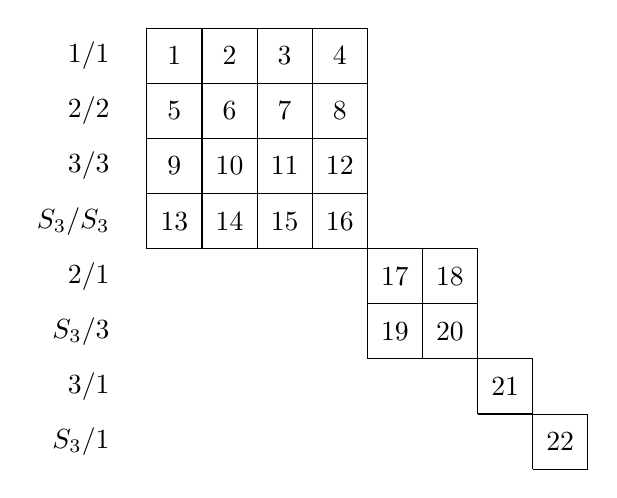
\begin{tikzpicture}[xscale=0.7,yscale=-0.7]
    \draw[shift={(0.5,0.5)}](0,0) grid (4,4);
    \draw[shift={(0.5,0.5)}](4,4) grid (6,6);
    \draw[shift={(0.5,0.5)}](6,6) grid (7,7);
    \draw[shift={(0.5,0.5)}](7,7) grid (8,8);
    \node[anchor=east] at (0,1) {$1/1$};
    \node[anchor=east] at (0,2) {$2/2$};
    \node[anchor=east] at (0,3) {$3/3$};
    \node[anchor=east] at (0,4) {$S_3/S_3$};
    \node[anchor=east] at (0,5) {$2/1$};
    \node[anchor=east] at (0,6) {$S_3/3$};
    \node[anchor=east] at (0,7) {$3/1$};
    \node[anchor=east] at (0,8) {$S_3/1$};
    \foreach \i in {1,...,16}
      \node[anchor=center] at ({mod(\i-1,4)+1}, {int((\i+3)/4)}) {$\i$};
    \foreach \i in {17,...,20}
      \node[anchor=center] at ({mod(\i-1,2)+5}, {int((\i-1)/2)-3}) {$\i$};
    \node[anchor=center] at (7, 7) {$21$};
    \node[anchor=center] at (8, 8) {$22$};
      \end{tikzpicture}
\end{center}

\begin{center}
  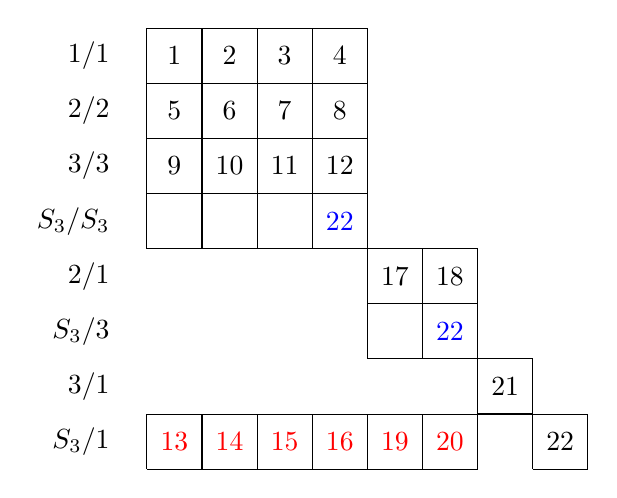
\begin{tikzpicture}[xscale=0.7,yscale=-0.7]
    \draw[shift={(0.5,0.5)}](0,0) grid (4,4);
    \draw[shift={(0.5,0.5)}](4,4) grid (6,6);
    \draw[shift={(0.5,0.5)}](6,6) grid (7,7);
    \draw[shift={(0.5,0.5)}](7,7) grid (8,8);
    \draw[shift={(0.5,0.5)}](0,7) grid (6,8);
    \node[anchor=east] at (0,1) {$1/1$};
    \node[anchor=east] at (0,2) {$2/2$};
    \node[anchor=east] at (0,3) {$3/3$};
    \node[anchor=east] at (0,4) {$S_3/S_3$};
    \node[anchor=east] at (0,5) {$2/1$};
    \node[anchor=east] at (0,6) {$S_3/3$};
    \node[anchor=east] at (0,7) {$3/1$};
    \node[anchor=east] at (0,8) {$S_3/1$};
    \foreach \i in {1,...,12}
      \node[anchor=center] at ({mod(\i-1,4)+1}, {int((\i+3)/4)}) {$\i$};
    \foreach \i in {13,...,16}
      \node[anchor=center] at ({mod(\i-1,4)+1}, {int((\i+3)/4)+4}) {\color{red} $\i$};
    \foreach \i in {17,18}
      \node[anchor=center] at ({mod(\i-1,2)+5}, {int((\i-1)/2)-3}) {$\i$};
    \foreach \i in {19,20}
      \node[anchor=center] at ({mod(\i-1,2)+5}, {int((\i-1)/2)-1}) {\color{red} $\i$};
    \node[anchor=center] at (7, 7) {$21$};
    \node[anchor=center] at (4, 4) {\color{blue} $22$};
    \node[anchor=center] at (6, 6) {\color{blue} $22$};
    \node[anchor=center] at (8, 8) {$22$};
      \end{tikzpicture}
\end{center}

Projective Resolutions:
\begin{align*}
P(1) \oplus P(2) \to P(S_3) \to P(1)  & \to S(1) \\
P(1) \oplus P(2) \to P(S_3) \to P(1)  & \to S(2) \\
P(3) & \to S(3) \\
P(1) \oplus P(2) \to P(S_3) & \to S(S_3)
\end{align*}

Decomposition/Cartan Matrix:
\begin{align*}
  D &= \left(
  \begin{array}{cccc}
    1&.&.&.\\
    .&1&.&.\\
    .&.&1&.\\
    1&1&.&1
  \end{array}
  \right)\text,&
C = D D^{\mathrm{tr}} &= \left(
  \begin{array}{cccc}
    1&.&.&1\\
    .&1&.&1\\
    .&.&1&.\\
    1&1&.&3
  \end{array}
  \right)\text,&
\det C &= 1\text.
\end{align*}

\end{document}
